\chapter{Background}
\label{chapterlabel1}
In this chapter we provide necessary background knowledge for understanding the content of this thesis. 
\section{N-gram Language Models}
In NLP, the \textbf{language models} are developed to compute the probability of a given sentence\cite{jurafsky2000speech}.
For example, a candidate sentence
\begin{center}
	``\emph{The cat sits on the mat.}''
\end{center}
A language model should assign a probability $p(\text{The cat sits on the mat})$ to this sentence.
We can treat the example sentence as a sequence of words, then $p(\text{The cat sits on the mat})$ becomes the joint probability of the terms in this sentence\cite{shannon2001mathematical}, and it is possible to factorise this joint probability by applying the chain rule of probability.
In our example, we have 6 words $\{w_{1} = \text{the}, w_{2} = \text{cat}, w_{3} = \text{sits}, w_{4} = \text{on}, w_{5}, \text{the}, w_{6} = \text{mat}\}$,before factorisation we add another two special tokens $w_{0} = <\text{s}>$,$w_{7} =<\backslash\text{s}>$ to indicate the begin and end of sentence. 
Now the probability assigned to this modified sentence becomes
\begin{equation}
p(w_{0:7}) = p(w_{0})\prod_{i=7}^{7}p(w_{i}|w_{1:i-1})
\end{equation}
\begin{equation}
p(w_{0}) = 1
\end{equation}
We can simplify the conditional distribution terms by assuming  that each word only depends on $n-1$ previous words so that
\begin{equation}
p(w_{i}|w_{1:i-1}) \approx p(w_{i}|w_{i-n+1:i-1})
\end{equation}
This yields to the wildly used \textbf{n-gram} language models in NLP\cite{jurafsky2000speech}, if we choose $n=2$, then we call this 2-gram model and so on.
If a training corpus (a collection of text documents) is available, 
we can compute the value of conditional distribution $p(w_{i}|w_{i-n+1:i-1})$ based on co-occurrence counts. For example, if we want to train a 2-gram model for the given corpus
\begin{center}
	``$<s>$ The cat sits on the mat $<\backslash s>$''\\
	``$<s>$ The cat sits on the desk $<\backslash s>$''
\end{center}
We can work out the conditional probabilities for instance $p(\text{cat}|\text{the})$ as
\begin{equation}
p(\text{cat}|\text{the}) = \frac{C(\text{the cat})}{C(\text{the})} = \frac{2}{4} = 0.5
\end{equation}
Where $C(\cdot)$ is the counts of token's occurrence in given corpus.
\begin{table}[H]
	\centering
	\begin{tabular}{c|c||c|c}
		\textbf{Vocabulary} ($\mathbf{V}$) & Occurrence& \textbf{2-grams} & Occurrence\\
		\hline
		$<s>$ & 2 &$<s>$ the& 2\\
		the & 4&the cat &2\\
		cat & 2&cat sits& 2\\
		sits &2 &sits on &2\\
		on &2& on the &2\\
		mat &1 &the mat &1\\
		desk &1 &the desk &1\\
		$<\backslash s>$ &2 &mat $<\backslash s>$&1\\
		-& - &desk $<\backslash s>$ &1 \\	
	\end{tabular}
	\caption{Occurrence for 2-gram and words of the example corpus}
\end{table}
\noindent
Having a language model like n-gram that can assign the probability to sentences is essential for many NLP tasks.
For example in \textbf{spelling correction}, a language model would assign a low probability to ``Their are two apples on the table'' because the word ``there'' is mistyped as ``their'',
this can help spelling checking model to detect errors\cite{jurafsky2000speech}. 
\begin{table}[H]
	\centering
	\begin{tabular}{c||cccccccc}
		& $<s>$ & the & cat & sits & on & mat & desk & $<\backslash s>$ \\
		\hline
		$<s>$ &0 & 0 & 0& 0 & 0& 0& 0 & 0\\
		the &0.5&0&0&0&0.5&0&0&0\\
		cat &0&1&0&0&0&0&0&0\\
		sits &0&0&1&0&0&0&0&0\\
		on &0&0&0&1&0&0&0&0\\
		mat &0&1&0&0&0&0&0&0\\
		desk &0&1&0&0&0&0&0&0\\
		$<\backslash s>$ &0&0&0&0&0&0.5&0.5&0\\
	\end{tabular}
	\caption{2-gram conditional probabilities for given example}
\end{table}
\noindent
The performance of n-gram increases with the training corpus size and n-gram size\cite{jurafsky2000speech,mikolov2012statistical}. 
However at same time, we have to spend huge amount of memory to store $p(w_{i}|w_{i-n+1:i-1})$ produce by n-gram if n and size of vocabulary $|\mathbf{V}|$ is to large, because the storage array requires $|\mathbf{V}|^{n}$ memory to store all possible $p(w_{i}|w_{i-n+1:i-1})$, and usually this array is very sparse (as shown in Table 2.2).
On the other hand, n-gram models only encode co-occurrence probabilities between words and grams. To capture additional information between words, for example, the semantic similarity we need to build a massive semantic network\cite{lehmann1992semantic} which can be very expensive to create and maintain.
Therefore we desire a model that can learn richer information from training corpus and requires cheaper storage when doing large scale language modelling.\\\\
Artificial neural networks are a family of machine learning methods, which have shown its ability to learn the dense and informative representations of input data\cite{bengio2009learning}. 
Thus many researchers have applied neural networks to learn representations for text data and solve NLP task, many of these applications have achieved remarkable results\cite{mikolov2012statistical}.  
Before we go further, we first provide some background knowledge about neural networks.
\section{Feedforward Neural Network}
\begin{figure}[h]
	\def\layersep{2.5cm}
	\begin{center}
		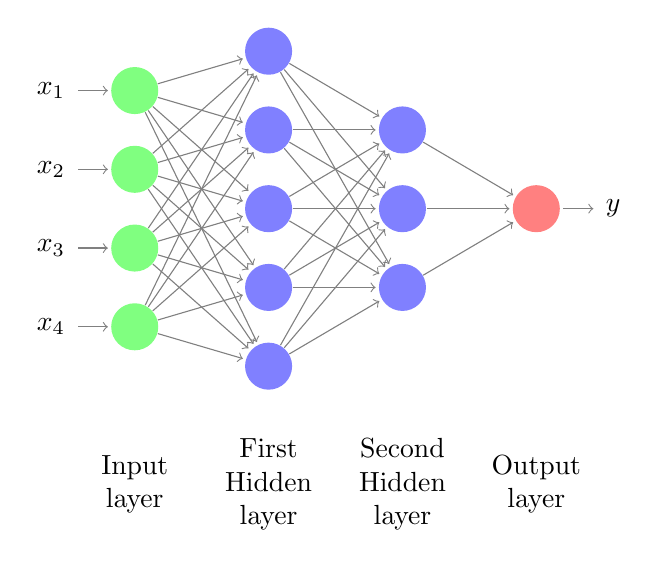
\begin{tikzpicture}[shorten >=1pt,->,draw=black!50, node distance=\layersep]
		\tikzstyle{every pin edge}=[<-,shorten <=1pt]
		\tikzstyle{neuron}=[circle,fill=black!25,minimum size=17pt,inner sep=0pt]
		\tikzstyle{input neuron}=[neuron, fill=green!50];
		\tikzstyle{output neuron}=[neuron, fill=red!50];
		\tikzstyle{hidden neuron}=[neuron, fill=blue!50];
		\tikzstyle{annot} = [text width=4em, text centered]
		
		% Draw the input layer nodes
		\foreach \name / \y in {1,...,4}
		% This is the same as writing \foreach \name / \y in {1/1,2/2,3/3,4/4}
		\node[input neuron, pin=left:$x_{\y}$] (I-\name) at (0,-\y) {};
		
		% Draw the hidden layer nodes
		\foreach \name / \y in {1,...,5}
		\path[yshift=0.5cm]
		node[hidden neuron] (H1-\name) at (\layersep,-\y cm) {};
		
		\foreach \name / \y in {2,...,4}
		\path[yshift = 0.5cm]
		node[hidden neuron] (H2-\name) at (\layersep*2,-\y cm) {};
		
		% Draw the output layer node
		\node[output neuron,pin={[pin edge={->}]right:$y$}, right of=H2-3] (O) {};
		
		% Connect every node in the input layer with every node in the
		% hidden layer.
		\foreach \source in {1,...,4}
		\foreach \dest in {1,...,5}
		\path (I-\source) edge (H1-\dest);
		
		% Connect every node in the hidden layer with the output layer
		\foreach \source in {1,...,5}
		\foreach \dest in {2,...,4}
		\path (H1-\source) edge (H2-\dest);
		
		\foreach \source in {2,...,4}
		\path (H2-\source) edge (O);
		
		% Annotate the layers
		\node[annot,below of=H1-5, node distance=1.5cm] (h1) {First Hidden layer};
		\node[annot,right of=h1] (h2) {Second Hidden layer};
		\node[annot,left of=h1] {Input layer};
		\node[annot,right of=h2] {Output layer};
		\end{tikzpicture}
	\end{center}
	\caption{ An example of deep feedforward network with 2 hidden layers}
\end{figure}
\noindent
A feedforward neural network defines a mapping function $ f(\mathbf{x},\mathbf{\theta})$ and tries to learn the value of parameters $\mathbf{\theta}$ result in the best approximation of the actual mapping $\mathbf{y} = f^{*}(\mathbf{x})$ between $\mathbf{y}$ and $\mathbf{x}$. 
For example, a chain like function $\mathbf{y}' = f^{3}(f^{2}(f^{1}(\mathbf{x})))$.
We usually call $f^{1}$ the \textbf{first hidden layer} of the network, $f^{2}$ the \textbf{second hidden layer} and so on. 
And we refer the final function $f^{3}$ as the \textbf{output layer} of neural network.
The number of layers gives the \textbf{depth} of the neural network. 
This is the terminology that the name \textbf{``deep learning"} arises\cite{Goodfellow2016Book}.
\subsection{Set up A Neural Network}
Training a supervised neural network $f(\mathbf{x},\mathbf{\theta})$ requires to define a loss function $L(\mathbf{y},f(\mathbf{x},\mathbf{\theta}))$ , where $\mathbf{y}$ is actual label of input $\mathbf{x}$.
In most cases, we follow the principle of maximum likelihood to train neural networks; that is to maximise the defined conditional distribution $p_{model}(\mathbf{y}|\mathbf{x})$. Usually, we use the cross entropy between the training data and model's predictions as the loss function\cite{Goodfellow2016Book}.
\begin{equation}
L(\mathbf{y},f(\mathbf{x},\mathbf{\theta})) = -\mathbb{E}_{\hat{p}_{data}} \log p_{model}(\mathbf{y}|\mathbf{x})
\end{equation}
Where the neural network $f(\mathbf{x},\mathbf{\theta})$ is trained to approach the conditional distribution $p_{model}(\mathbf{y}|\mathbf{x})$. 
For $f(\mathbf{x},\mathbf{\theta})$ to be a valid probability distribution, the output of  $f(\mathbf{x},\mathbf{\theta})$ must within $[0,1]$. \\\\
In many tasks, the neural network is required to make a binary prediction of variable $y \in \{0,1\} $. In this case, a convenient choice of the output layer for the neural network is the sigmoid function. For example, we can define a very simple neural network with sigmoid output layer as
\begin{equation}
f(\mathbf{\theta},\mathbf{x}) = \sigma(\mathbf{\theta}^{T}\mathbf{x}) = \frac{1}{1+\exp({-\mathbf{\theta}^{T}\mathbf{x}})}
\label{sigmoid}
\end{equation}
Where the first hidden layer is the inner product of $\mathbf{\theta}$ and $\mathbf{x}$, and the output layer is the sigmoid function. 
Our cross entropy loss function is 
\begin{equation}
L(y,f(\mathbf{x},\mathbf{\theta})) = y\log f(\mathbf{x},\mathbf{\theta}) + (1-y)\log(1-f(\mathbf{x},\mathbf{\theta}))
\end{equation}
And we usually make our prediction $\hat{y}$ by
\begin{equation}
y' = \begin{cases}
0 & \text{if } f(\mathbf{\theta},\mathbf{x}) > 0.5\\
1 & \text {if } f(\mathbf{\theta},\mathbf{x}) \leq 0.5 \\
\end{cases}
\end{equation}\\\\
When solving the multiple classes classification problems, for example, a three types classification problem, the actual label $\mathbf{y}$ is usually a one-hot vector, which can be
\begin{equation}
\mathbf{y} = \begin{bmatrix}
1\\
0\\
0\\
\end{bmatrix}
\end{equation}
To perform this task the output layer is required to assign a probability to each class, and the sum of assigned probabilities must equal to 1.
\begin{equation}
f(\mathbf{x},\mathbf{W}) =\begin{bmatrix}
p_{1} \\
p_{2} \\
p_{3} \\
\end{bmatrix}
\end{equation}
\begin{equation}
\sum_{i=1}^{3} p_{i} = 1
\end{equation}
A common choice of output layer for multiple classes classification problems is softmax function, the softmax function assigns a probability to each element as
\begin{equation}
p_{i} = \frac{\exp\{\mathbf{w}_{i}^{T} \mathbf{x}\}}{\sum_{i=1}^{3}\exp\{\mathbf{w}_{i}^{T} \mathbf{x}\}}
\end{equation}
Where we define
\begin{equation}
\mathbf{Wx} = \begin{bmatrix}
\mathbf{w}_{1}^{T}\\
\mathbf{w}_{2}^{T}\\
\mathbf{w}_{3}^{T}\\
\end{bmatrix} \mathbf{x}
\end{equation}
The loss function in this case is  
\begin{equation}\label{softmax_loss}
L(\mathbf{y},f(\mathbf{x},\mathbf{W})) = \sum_{i=1}^{3}y_{i}\log p_{i}
\end{equation}
In our example, because we know in advance that all the elements of $\mathbf{y}$ is 0 except the first one, so the Equation \ref{softmax_loss} can be reduced to 
\begin{equation}
L(\mathbf{y},f(\mathbf{x},\mathbf{W})) = y_{1}\log p_{1}
\end{equation}
If the output we obtain from $f(\mathbf{x},\mathbf{W})$ is 
\begin{equation}
f(\mathbf{x},\mathbf{W}) = \begin{bmatrix}
p_{1} \\
p_{2} \\
p_{3} \\
\end{bmatrix} = \begin{bmatrix}
0.3 \\
0.5 \\
0.2\\
\end{bmatrix}
\end{equation}
We can make our prediction $\mathbf{y}'$ by convert the element with maximum probability $p_{i}$ to 1, and others to 0.
\begin{equation}
\mathbf{y} = \begin{bmatrix}
0\\
1\\
0 \\
\end{bmatrix}
\end{equation}
\subsection{Gradient Based Learning}
Once we have a training set $D = \{\mathbf{x}_{1:n},\mathbf{y}_{1:n}\}$, the neural network $f(\mathbf{x},\mathbf{\theta}))$ and loss function $L(\mathbf{y},f(\mathbf{x},\mathbf{\theta}))$, we are facing the problem of learning optimal parameters $\mathbf{\theta}^{*}$ to minimise loss function.
\begin{equation}
\mathbf{\theta}^{*} = \arg\min_{\mathbf{\theta}}L(\mathbf{y},f(\mathbf{x},\mathbf{\theta}))
\end{equation}
The neural networks are trained to learn optimal parameters $\mathbf{\theta}^{*}$ by iterative gradient based algorithms. 
For example, the \textbf{Gradient Descent} (GD)
\begin{algorithm}[H]
	initialise $\gamma$ \\
	randomly initialise $\mathbf{\theta} \gets \mathbf{\theta}_{0}$ \\
	\While{Stop criteria not meet}{
		$\mathbf{\theta}\gets \mathbf{\theta} - \frac{\gamma}{|D|}\sum_{i=1}^{|D|} \bigtriangledown_{\mathbf{\theta}} L(\mathbf{y}_{i},f(\mathbf{x}_{i},\mathbf{\theta}))$ \\
	} 
	$\mathbf{\theta}^{*} \gets \mathbf{\theta}$
	\caption{GD for finding $\mathbf{\theta}^{*}$}
\end{algorithm}
\noindent
The $\gamma$ is known as learning rate, which controls the speed of gradients update. $|D|$ is the size of the training dataset. 
The stop criteria can vary with different training strategies, one simple choice of stop criteria is to limit the maximum number of iterations.

\begin{algorithm}[H]
	initialize $\gamma$ \\
	initialize $\mathbf{\theta} \gets \mathbf{\theta}_{0}$ \\
	\While{Stop criteria not meet}{
		Sample a minibatch $\{(\mathbf{x}_{1},\mathbf{y}_{1}), ..., (\mathbf{x}_{s},\mathbf{y}_{s})\}$ from $D$ \\
		$\mathbf{g} \gets \frac{1}{s} \sum_{i=1}^{s} \bigtriangledown_{\mathbf{\theta}} L(\mathbf{y}_{i},f(\mathbf{x}_{i},\mathbf{\theta}))$ \\
		$\mathbf{\theta} \gets \mathbf{\theta} - \gamma \mathbf{g}$ \\} 
	$\mathbf{\theta}^{*} \gets \mathbf{\theta}$
	\caption{Basic SGD algorithm for finding $\mathbf{\theta}^{*}$}
\end{algorithm}
\noindent
Apply GD has to iterate through the whole training dataset for single step gradients update when the size of training dataset is large GD can be very computationally expensive.
Unlike GD, \textbf{Stochastic Gradient Descent} (SGD) computes the approximated gradients based on a random minibatch (a subset) sampled from training data $D$, and it terms out that SGD tends to work better than GD on a large dataset\cite{Goodfellow2016Book}. \\\\
There are many extended versions of SGD algorithms which can result in better and faster convergence, readers who are interested in can refer to \cite{kingma2014adam,sutskever2013importance}. \\\\
In above discussion, we only introduce different gradient based algorithms for parameters update. 
To apply these algorithms, we need a mechanism that can compute gradients.
Here we briefly introduce the \textbf{back propagation} algorithm\cite{rumelhart1988learning} which can efficiently compute exact gradients for any differentiable functions.
The back propagation algorithm is based on the chain rule of calculus, let $x$ be a scalar real number, and suppose we have $y = g(x)$ and $z=f(y)$. Then the chain rule gives that
\begin{equation}
\frac{dz}{dx} = \frac{dz}{dy}\frac{dy}{dx}
\end{equation}
Now consider the following function 
\begin{equation}
f(x_{1},x_{2}) = \cos(\exp((x_{1}x_{2}))
\end{equation}
Figure \ref{2.2a} gives a graph illustrate of this function.
Refer to Figure \ref{2.2a}, to calculate the derivative of $f(\cdot)$ with respected to $x_{1}$ and $x_{2}$, we need to evaluate
\begin{equation}\label{x_1}
\frac{df}{dx_{1}} = \frac{df_{3}}{df_{2}}\frac{df_{2}}{df_{1}}\frac{df_{1}}{dx_{1}}
\end{equation}
and
\begin{equation}\label{x_2}
\frac{df}{dx_{2}} = \frac{df_{3}}{df_{2}}\frac{df_{2}}{df_{1}}\frac{df_{1}}{dx_{2}}
\end{equation}
We could compute $\frac{df}{dx_{1}}$ and $\frac{df}{dx_{2}}$ by forward propagating (Figure \ref{2.2b}) or backward propagating (Figure \ref{2.2c}) the intermediate derivatives. 
We can notice that there is a shared path between $\frac{df}{dx_{1}}$ and $\frac{df}{dx_{2}}$ which is 
\begin{equation}
\frac{df_{3}}{df_{1}} = \frac{df_{3}}{df_{2}}\frac{df_{2}}{df_{1}}  
\end{equation}
By doing the backward gradient propagation, we do not need to recompute $\frac{df_{3}}{df_{1}}$, while forward propagation has to.
This makes the forward propagation requires 2 more evaluations to work out $\frac{df}{dx_{1}}$ and $\frac{df}{dx_{2}}$ compares with back propagation in our example.
Research suggests that the complexity of back propagation is approximately equal to the complexity of evaluating $f(\cdot)$, while the complexity of calculating derivatives forward is $n$ times greater\cite{naumann2012art}, where $n$ is the numbers of inputs of $f(\cdot)$.
\begin{figure*}[h]
	\centering
	\begin{subfigure}[t]{0.3\textwidth}
		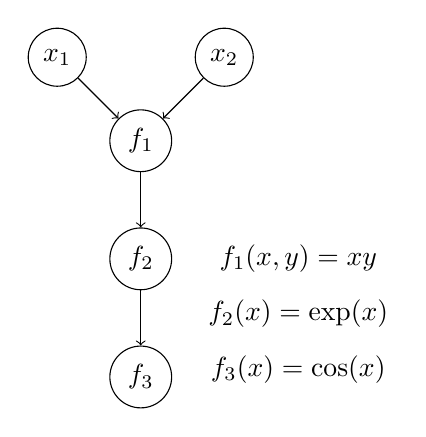
\begin{tikzpicture}
		\node[circle,draw,node distance=15mm](multi){$f_{1}$};
		\node[circle,draw, node distance=15mm,above left of=multi](x1){$x_{1}$};
		\node[circle,draw,above right of=multi,node distance=15mm](x2){$x_{2}$};
		\node[circle,draw,below of =multi,node distance=15mm](exp){$f_{2}$};
		\node[circle,draw,below of =exp,node distance=15mm](cos){$f_{3}$};
		\node[right of=exp,node distance=20mm](formula1){$f_{1}(x,y)=xy$};
		\node[below of=formula1,node distance=7mm](formula2){$f_{2}(x)=\exp(x)$};
		\node[below of=formula2,node distance=7mm](formula3){$f_{3}(x)=\cos(x)$};
		\path[->]
		(x1) edge (multi)
		(x2) edge (multi)
		(multi) edge (exp)
		(exp) edge (cos);
		\end{tikzpicture}
		\caption{The computational graph for evaluating $f(\cdot)$}
		\label{2.2a}
	\end{subfigure}%
	~	
	\begin{subfigure}[t]{0.3\textwidth}
		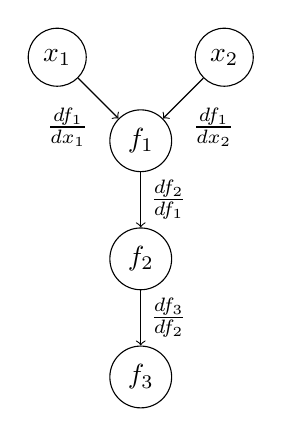
\begin{tikzpicture}[node distance=15mm]
		\node[circle,draw](multi){$f_{1}$};
		\node[circle,draw, above left of=multi](x1){$x_{1}$};
		\node[circle,draw,above right of=multi](x2){$x_{2}$};
		\node[circle,draw,below of =multi](exp){$f_{2}$};
		\node[circle,draw,below of =exp](cos){$f_{3}$};
		\path[->]
		(x1) edge node[below left] {$\frac{d f_{1}}{d x_{1}}$} (multi)
		(x2) edge node[below right] {$\frac{d f_{1}}{d x_{2}}$}(multi)
		(multi) edge node[right] {$\frac{d f_{2}}{d f_{1}}$} (exp)
		(exp) edge node[right] {$\frac{d f_{3}}{d f_{2}}$}(cos);
		
		\end{tikzpicture}
		\caption{The forward propagation of derivatives}
		\label{2.2b}
	\end{subfigure}
	~	
	\begin{subfigure}[t]{0.3\textwidth}
		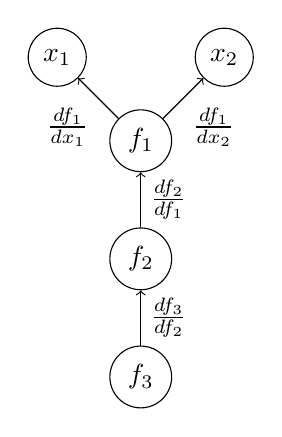
\begin{tikzpicture}[node distance=15mm]
		\node[circle,draw](multi){$f_{1}$};
		\node[circle,draw, above left of=multi](x1){$x_{1}$};
		\node[circle,draw,above right of=multi](x2){$x_{2}$};
		\node[circle,draw,below of =multi](exp){$f_{2}$};
		\node[circle,draw,below of =exp](cos){$f_{3}$};
		\path[->]
		(multi) edge node[below left] {$\frac{d f_{1}}{d x_{1}}$} (x1)
		(multi) edge node[below right] {$\frac{d f_{1}}{d x_{2}}$}(x2)
		(exp) edge node[right] {$\frac{d f_{2}}{d f_{1}}$} (multi)
		(cos) edge node[right] {$\frac{d f_{3}}{d f_{2}}$}(exp);
		\end{tikzpicture}
		\caption{The backward propagation of derivatives}
		\label{2.2c}
	\end{subfigure}
	\caption{An diagram illustration of computing the value of $f(x_{1},x_{2})$ and its derivatives, we can see that, to calculate the result of $f(\cdot)$, we need 3 evaluation steps (Figure \ref{2.2a}).
		And for the gradients $\frac{df}{dx_{1}}$ and $\frac{df}{dx_{2}}$, we need 6 evaluations for forward propagation (Figure \ref{2.2b}) and 4 evaluations for backward propagation (Figure \ref{2.2c}). }
\end{figure*}

\noindent
The above example only shows the basic idea of back propagation algorithm. There are many deep learning packages for example Theano\cite{2016arXiv160502688short} and Tensorflow\cite{tensorflow2015-whitepaper}, implemented back-propagation algorithm to compute gradients for training neural networks.
\section{Regularisation}
When training a neural network, we usually incur the problem of \textbf{overfitting}. 
There are many regularisation methods explicitly designed to reduce overfitting during training time. Here we introduce two methods we will use in this thesis.\\\\
\textbf{$L^{2}$ regularisation} which also known as weight decay, is the simplest and most commonly used regularisation method. 
Assume that $\mathbf{\theta}$ stands for the parameters of the neural network, and the loss function is $L_{\mathbf{\theta}}$. 
To perform the $l^{2}$ regularisation, we add $l^{2}$ norm of $\mathbf{\theta}$ and loss function, then minimise them together with respect to $\mathbf{\theta}$
\begin{equation}
J = L_{\mathbf{\theta}} + \frac{\alpha}{2}||\mathbf{\theta}||_{2}^{2}
\end{equation}
Where $\alpha$ controls the importance of regularisation term.

\begin{algorithm}[H]
	early stop trigger $p$  \\
	updating step $n$\\
	initialize $\gamma$ \\
	integer counter $j \gets 0$\\
	optimal parameters $\mathbf{\theta}^{*} \gets \mathbf{0}$\\
	initialize $v \gets \infty$ \\
	initialize $\mathbf{\theta} \gets \mathbf{\theta}_{0}$ \\
	\While{$j < p$}{
		\For{$0$ to n}{
			Sample a minibatch $\{(\mathbf{x}_{1},\mathbf{y}_{1}), ..., (\mathbf{x}_{s},\mathbf{y}_{s})\}$ from $D$ \\
			$\mathbf{g} \gets \frac{1}{s} \sum_{i=1}^{s} \bigtriangledown_{\mathbf{\theta}} L(\mathbf{y}_{i},f(\mathbf{x}_{i},\mathbf{\theta}))$ \\
			$\mathbf{\theta} \gets \mathbf{\theta} - \gamma \mathbf{g}$ \\
		}
		Get validation set $V$\\
		$v' \gets \frac{1}{|V|}\sum_{(\mathbf{x}_{i},\mathbf{y}_{i} \in V)}L(\mathbf{y}_{i},f(\mathbf{x}_{i},\mathbf{\theta}))$\\
		$j++$ \\
		\If{$v' < v$}{
			$j \gets 0$ \\
			$v \gets v'$ \\
			$\mathbf{\theta}^{*} \gets \mathbf{\theta}$\\
		} }
		\textbf{return} $\mathbf{\theta}^{*}$
		\caption{SGD with early stopping}
	\end{algorithm}
\newpage
\noindent
When training a neural network, it is common to use a validation set to estimate generalisation error during training.
If the neural network starts to overfit, we usually observe that training error decreases steadily over time, while the error on validation set starts to rise again. 
This means that we can obtain $\mathbf{\theta}$ with better generalisation error by storing $\mathbf{\theta}$ at the point with the lowest validation error,
and hope this $\mathbf{\theta}$ can also perform well on testing set.
This strategy is known as \textbf{early stopping}.\\\\
When applying the early stopping, our stop criteria depends on validation loss.
In the given example (Algorithm 3), we use an integer counter $j$ to record the number of times that validation loss increases.
$j$ is always set to 0 if the validation loss is decreasing.
When $j$ is greater or equal to our maximum number of allowance $p$, we halt the algorithm and return $\mathbf{\theta}$\cite{Goodfellow2016Book}.


\section{Recurrent Neural Networks}
	\begin{figure*}[h]
		\centering
		\begin{subfigure}[t]{0.35\textwidth}
			\centering
			\usetikzlibrary{arrows}
			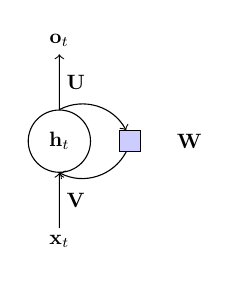
\begin{tikzpicture}[scale=0.75, every node/.style={scale=0.75}]
			\tikzstyle{neuron}=[circle,minimum size=3em]
			\def\layersep{1.7cm}
			\node[](input) at (8 cm, -\layersep*2){$\mathbf{x}_{t}$};
			\node[neuron,draw](hidden) at(8 cm, -\layersep){$\mathbf{h}_{t}$};
			\node[](output) at (8 cm, 0 cm) {$\mathbf{o}_{t}$};
			\node[draw,fill=blue!20,minimum size = 1em,right of=hidden,node distance=12mm](recurrent){}
			edge[->,bend left=45](hidden.south)
			edge[<-,bend right=45](hidden.north);
			\node[right of=recurrent]{$\mathbf{W}$};
			\path[->] (input) edge node[right]{$\mathbf{V}$} (hidden)
			(hidden) edge node[right]{$\mathbf{U}$} (output);
			\end{tikzpicture}
			\caption{A folded RNN update graph}
			\label{folded}
		\end{subfigure}
		~
		\begin{subfigure}[t]{0.6\textwidth}
			\centering
			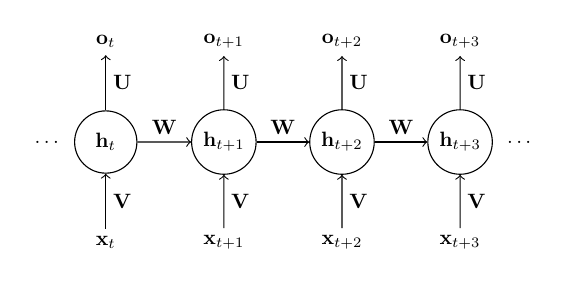
\begin{tikzpicture}[scale=0.75, every node/.style={scale=0.75}]
			\def\layersep{1.7cm}
			\tikzstyle{neuron}=[circle,minimum size=3em]
			\node[](i-t) at (0 cm, -\layersep*2){$\mathbf{x}_{t}$};
			\node[neuron,draw](h-t) at(0 cm, -\layersep){$\mathbf{h}_{t}$};
			\node[](o-t) at (0 cm, 0 cm) {$\mathbf{o}_{t}$};
			
			\foreach  \y in {3,...,1}
			\node[neuron,draw](h-\y)at (\y*2 cm,-\layersep) {$\mathbf{h}_{t+\y}$};
			
			\foreach \y in {1,...,3}
			\node[](o-\y) at (\y*2 , 0 cm){$\mathbf{o}_{t+\y}$};
			
			\foreach \y in {1,...,3}
			\node[](i-\y)at (\y*2 cm,-\layersep*2) {$\mathbf{x}_{t+\y}$};
			
			\node[left of=h-t](h-before){$\dots$};
			\node[right of=h-3](h-after){$\dots$};
			
			\foreach \y in {1,...,3}
			\path[->] (i-\y) edge node[right]{$\mathbf{V}$} (h-\y);
			\foreach \y in {1,...,3}
			\path[->] (h-\y) edge node[right]{$\mathbf{U}$} (o-\y);
			
			\path[->] (i-t) edge node[right]{$\mathbf{V}$} (h-t)
			(h-t) edge node[right]{$\mathbf{U}$} (o-t)
			(h-t) edge node[above]{$\mathbf{W}$} (h-1)
			(h-1) edge node[above]{$\mathbf{W}$} (h-2)
			(h-2) edge node[above]{$\mathbf{W}$} (h-3);
			\end{tikzpicture}
			\caption{An unfolded update graph of RNN}
			\label{unfolded}
		\end{subfigure}
		\caption{A simple diagram example of RNN architecture, the parameters $\mathbf{U,V,W}$ are shared across the model. At each time step, the hidden state is computed based on the current input and previous hidden state}
	\end{figure*}
	
	\noindent
\textbf{Recurrent neural networks} (RNNs) are neural networks that can process sequential data. 
An important property of RNNs is that the parameters are shared across the model\cite{elman1991distributed}. 
This makes RNN possible to take input sequences with arbitrary length and generalise across them.
Here we give an example of a simple RNN, which contains a single and self-connected hidden layer.
	\begin{equation}\label{eq:ht}
	\mathbf{h}_{t} = \tanh(\mathbf{V}\mathbf{x}_{t} + \mathbf{W}\mathbf{h}_{t-1})
	\end{equation}
	\begin{equation}\label{eq:yt}
	\mathbf{o}_{t} = \text{softmax}(\mathbf{U}\mathbf{h}_{t})
	\end{equation}
A convenient way to visualise RNN is to consider the unfolded parameter update graph of the network along with the input sequence, Figure \ref{unfolded} shows part of an unfolded RNN\cite{Goodfellow2016Book}.
We can see that, each hidden state $\mathbf{h}_{t}$ can capture the information from past $\mathbf{h}_{t-1}$ and present input $\mathbf{x}_{t}$. 
So we can consider the last hidden as a ``summary'' of input sequence. 
	\begin{figure*}[h]
		\centering
		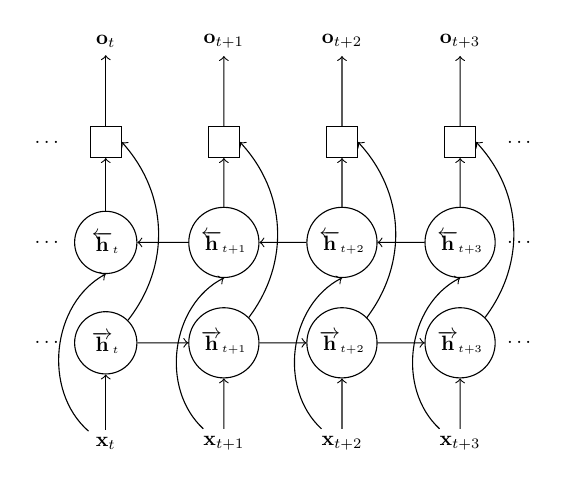
\begin{tikzpicture}[scale=0.75, every node/.style={scale=0.75}]
		\def\layersep{1.7cm}
		\tikzstyle{neuron}=[circle,minimum size=3em]
		\node[](i-t) at (0 cm, -\layersep*4){$ \mathbf{x}_{t}$};
		
		\node[neuron,draw](bh-t) at(0 cm, -\layersep*2){$ \scriptstyle  \overleftarrow{\mathbf{h}}_{t}$};
		
		\node[neuron,draw](fh-t) at(0 cm, -\layersep*3){$\scriptstyle \overrightarrow{\mathbf{h}}_{t}$};
		
		\node[draw,fill=white,minimum size = 1.5em](con-t)at (0 cm,-\layersep) {};
		
		\node[](o-t) at (0 cm, 0 cm) {$ \mathbf{o}_{t}$};
		
		\foreach \y in {1,...,3}
		\node[](i-\y)at (\y*2 cm,-\layersep*4) {$ \mathbf{x}_{t+\y}$};
		
		
		\foreach  \y in {3,...,1}
		\node[neuron,draw](bh-\y)at (\y*2 cm,-\layersep*2) {$\scriptstyle \overleftarrow{\mathbf{h}}_{t+\y}$};
		
		\foreach  \y in {3,...,1}
		\node[neuron,draw](fh-\y)at (\y*2 cm,-\layersep*3) {$\scriptstyle \overrightarrow{\mathbf{h}}_{t+\y}$};
		
		\foreach  \y in {3,...,1}
		\node[draw,fill=white,minimum size = 1.5em](con-\y)at (\y*2 cm,-\layersep) {};
		
		\foreach \y in {1,...,3}
		\node[](o-\y) at (\y*2 , 0 cm){$ \mathbf{o}_{t+\y}$};
		
		\node[left of=fh-t](fh-before){$\dots$};
		\node[right of=fh-3](fh-after){$\dots$};
		\node[left of=bh-t](bh-before){$\dots$};
		\node[right of=bh-3](bh-after){$\dots$};
		\node[left of=con-t](con-before){$\dots$};
		\node[right of=con-3](con-after){$\dots$};
		
		\foreach \y in {1,...,3}
		\path[->] (i-\y) edge (fh-\y);
		\foreach \y in {1,...,3}
		\path[->] (bh-\y) edge (con-\y);
		\foreach \y in {1,...,3}
		\path[->] (con-\y) edge (o-\y);
		\foreach \y in {1,...,3}
		\path[->,bend left=55] (i-\y) edge (bh-\y.south);
		\foreach \y in {1,...,3}
		\path[->,bend right=40] (fh-\y) edge (con-\y.east);
		
		\path[->] (i-t) edge (fh-t)
		(bh-t) edge (con-t)
		(con-t) edge (o-t)
		(fh-1) edge (fh-2)
		(fh-2) edge (fh-3)
		(fh-t) edge (fh-1)
		(bh-3) edge (bh-2)
		(bh-2) edge (bh-1)
		(bh-1) edge (bh-t);
		\path[->,bend left=55] (i-t) edge (bh-t.south);
		\path[->,bend right=40] (fh-t) edge (con-t.east);
		\end{tikzpicture}
		\caption{A digram illustration of Bidirectional RNN, in this diagram the square box represents any transformation that can map forward and backward information into output.}
		\label{Bidir}
	\end{figure*}
	
	\noindent
	    In some situations, we may also want $\mathbf{h}_{t}$ to have information about future. 
	    The Bidirectional RNN\cite{schuster1997bidirectional} is proposed to address this need.
	    Acorrding to Figure \ref{Bidir}, the bottom RNN encodes past information into hidden state $\overrightarrow{\mathbf{h}}_{t}$, while the top RNN encodes future information hidden state $\overleftarrow{\mathbf{h}}_{t}$.
	The output at each time step is computed based on hidden states of both RNNs.  
\subsection{Back Propagation Through Time}
A common approach to determine the derivatives of RNN is Backpropagation Through Time (BPTT)\cite{werbos1990backpropagation}. 
Similar to standard back propagation, BPTT consists of a repeated application of chain rule. 
The difference is that to obtain correct gradients update of hidden layer parameters, we have to propagate the gradient all the way back to initial time step, as shown in Figure \ref{fig:BPTT}. 
	To be more specific, assume that we have an RNN based on Equation \ref{eq:ht} and Equation \ref{eq:yt}, the loss at time step t is $L_{t}(\mathbf{y}_{t},\mathbf{o}_{t})$ and we wish to update our parameter just base on $L_{t}(\mathbf{y}_{t},\mathbf{o}_{t})$.
	From Equation \ref{eq:ht} we can notice that, there is a recursive dependency between each hidden states and $\mathbf{W},\mathbf{V}$.
	So when doing the gradients update, we have to work out gradients at each time step, and sum all corresponding gradients to obtain correct update, here we only show the update of $\mathbf{W}$ as example
	\begin{equation}\label{BPTT}
	\frac{\partial L_{t}}{\partial \mathbf{W}} = \sum_{i=1}^{t}\frac{\partial L_{t}}{\partial\mathbf{o}_{t}}\frac{\partial \mathbf{o}_{t}}{\partial \mathbf{h}_{t}}(\prod_{j=i+1}^{t}\frac{\partial \mathbf{h}_{j}}{\partial \mathbf{h}_{j-1}})\frac{\partial \mathbf{o}_{i}}{\partial \mathbf{W}}
	\end{equation}
	From Equation \ref{BPTT} we can find that the hidden state Jacobian matrices are accumulating through time
	\[\frac{\partial \mathbf{h}_{t}}{\partial \mathbf{h}_{i}} = \prod_{j=i+1}^{t}\frac{\partial \mathbf{h}_{j}}{\partial \mathbf{h}_{j-1}}\]
	With t goes large ($t \rightarrow \infty$), $\frac{\partial \mathbf{h}_{t}}{\partial \mathbf{h}_{i}}$ can quickly shrink to zero or explode to infinity\cite{pascanu2013difficulty}. This can disrupt gradient update and results in the problem of learning long-term dependencies in RNN\cite{bengio1994learning}.
	\begin{figure*}[h]
		\centering
		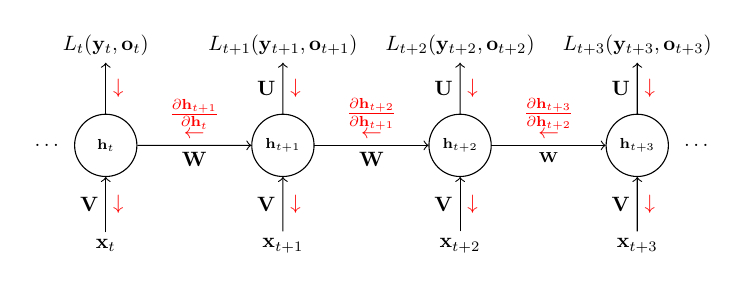
\begin{tikzpicture}[scale=0.75, every node/.style={scale=0.75}]
		\def\layersep{1.7cm}
		\tikzstyle{neuron}=[circle,minimum size=3em]
		\node[fill=white,minimum size=1em](i-t) at (0 cm, -\layersep*2){$\mathbf{x}_{t}$};
		\node[neuron,draw](h-t) at(0 cm, -\layersep){$\scriptstyle\mathbf{h}_{t}$};
		\node[fill=white,minimum size=1em](o-t) at (0 cm, 0 cm) {$L_{t}(\mathbf{y}_{t},\mathbf{o}_{t})$};
		
		\foreach  \y in {3,...,1}
		\node[neuron,draw](h-\y)at (\y*3 cm,-\layersep) {$\scriptstyle\mathbf{h}_{t+\y}$};
		
		\foreach \y in {1,...,3}
		\node[](o-\y) at (\y*3 , 0 cm){$L_{t+\y}(\mathbf{y}_{t+\y},\mathbf{o}_{t+\y})$};
		
		\foreach \y in {1,...,3}
		\node[](i-\y)at (\y*3 cm,-\layersep*2) {$\mathbf{x}_{t+\y}$};
		
		\node[left of=h-t](h-before){$\dots$};
		\node[right of=h-3](h-after){$\dots$};
		
		\foreach \y in {1,...,3}
		\path[->] (i-\y) edge node[left]{$\mathbf{V}$} node[right]{\textcolor{red}{$\downarrow$}} (h-\y);
		\foreach \y in {1,...,3}
		\path[->] (h-\y) edge node[left]{$\mathbf{U}$}node[right]{\textcolor{red}{$\downarrow$}} (o-\y);
		
		\path[->] (i-t) edge node[left]{$\mathbf{V}$} node[right]{\textcolor{red}{$\downarrow$}} (h-t)
		(h-t) edge node[right]{\textcolor{red}{$\downarrow$}} (o-t)
		(h-t) edge node[below]{$\mathbf{W}$} node[above]{\textcolor{red}{$\leftarrow$}}node[shift={(0em,1.5em)}]{\textcolor{red}{$\frac{\partial \mathbf{h}_{t+1}}{\partial \mathbf{h}_{t}}$}}  (h-1)
		(h-1) edge node[below]{$\mathbf{W}$}node[above]{\textcolor{red}{$\leftarrow$}}node[shift={(0em,1.5em)}]{\textcolor{red}{$\frac{\partial \mathbf{h}_{t+2}}{\partial \mathbf{h}_{t+1}}$}} (h-2)
		(h-2) edge node[below]{$\scriptstyle\mathbf{W}$} node[shift={(0em,1.5em)}]{\textcolor{red}{$\frac{\partial \mathbf{h}_{t+3}}{\partial \mathbf{h}_{t+2}}$}}  node[above]{\textcolor{red}{$\leftarrow$}}(h-3);
		\end{tikzpicture}
		\caption{A diagram illustration of BPTT on RNN, we can see that the partial derivatives between hidden states are accumulating back through time.
			As shown in this diagram, because the parameters of RNN are shared across, therefore in order to compute correct gradients update, we have to back propagate derivatives all the way back to initial time step.}
		\label{fig:BPTT}
	\end{figure*}
\subsection{Gated RNNs}
Using the gated RNNs is one effective way that can reduce the difficulty of learning long-term dependencies.
Gated RNNs produce paths through time that have derivatives neither vanish nor explode. An example of gated RNNs is \text{Gated Recurrent Units} (GRU)\cite{chung2014empirical},
in GRU the update equations for hidden unit $\mathbf{h}_{t}$ are
	\begin{equation}
	\mathbf{h}_{t} = \mathbf{u}_{t}\odot\mathbf{h}_{t-1} + (1-\mathbf{u}_{t})\odot \tilde{\mathbf{h}}_{t}
	\end{equation}
	Where $\mathbf{r}_{t}$ stands for ``reset'' gate and $\mathbf{u}_{t}$ for ``update'' gate, $\tilde{\mathbf{h}}_{t}$ is the candidate hidden state
	\begin{equation}
	\tilde{\mathbf{h}}_{t} = \tanh(\mathbf{W}\mathbf{x}_{t} + \mathbf{U}\begin{bmatrix}
	\mathbf{r}_{t}\odot\mathbf{h}_{t-1}
	\end{bmatrix} + b_{h})
	\end{equation}
	\begin{equation}
	\mathbf{u}_{t} = \sigma(\mathbf{W}_{u}\mathbf{x}_{t} + \mathbf{U}_{u}\mathbf{h}_{t-1} + b_{u})
	\end{equation}
	\begin{equation}
	\mathbf{r}_{t} = \sigma(\mathbf{W}_{r}\mathbf{x}_{t}+\mathbf{U}_{r}\mathbf{h}_{t-1}+b_{r})
	\end{equation}
	The reset gate can control information from past used to compute next target state, while update gate can ``copy'' the past or ``ignore'' it by replace it new target state.	
\begin{figure*}[h]
		\centering
		\usetikzlibrary{shapes,arrows}
		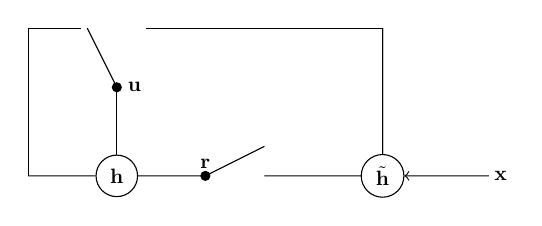
\begin{tikzpicture}[scale=0.75, every node/.style={scale=0.75}]
		\tikzstyle{neuron}=[circle,minimum size=2em]
		\node[neuron,draw](n1)at(0,-2){$\mathbf{h}$};
		\node[neuron,draw](n2)at(4.5,-2){$\tilde{\mathbf{h}}$};
		\draw[fill=black] (1.5,-2) circle (.5ex);
		\draw[fill=black] (0,-0.5) circle (.5ex);
		\draw[]{
			(n1.east) -- (1.5,-2)
		};
		\draw[]{
			(1.5,-2) -- (2.5,-1.5)
		};
		\draw[]{
			(2.5,-2) -- (n2.west)
		};
		\draw[]{
			(n1.north) --(0,-0.5)
		};
		\draw[]{
			(0,-0.5) -- (-0.5,0.5)
		};
		\draw[]{
			(-0.6,0.5) -- (-1.5,0.5)
		};
		\draw[]{
			(-1.5,0.5) --(-1.5,-2)
		};
		\draw[]{
			(-1.5,-2) -- (n1.west)
		};
		\draw[]{
			(0.5,0.5) -- (4.5,0.5)
		};
		\draw[]{
			(n2.north) --(4.5,0.5)
		};
		\node[](x)at(6.5,-2){$\mathbf{x}$};
		\node[](r)at(1.5,-1.8){$\mathbf{r}$};
		\node[](u)at(0.3,-0.5){$\mathbf{u}$};
		\path[->] (6.3,-2) edge (n2.east);
		\draw[]{
			(n2.north) --(4.5,0.5)
		};
		\end{tikzpicture}
		\caption{A simplified diagram illustration of GRU unit the update of $\mathbf{h}$,$\tilde{\mathbf{h}}$ is controlled by $\mathbf{r}$ and $\mathbf{u}$.}
	\end{figure*}
	\section{Autoenocder}
	\begin{figure*}[h]
		\centering
		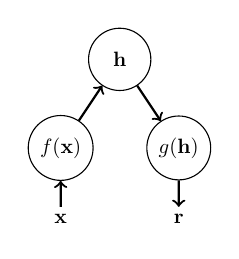
\begin{tikzpicture}[scale=0.75, every node/.style={scale=0.75}]
		\tikzstyle{neuron}=[circle,minimum size=3em]
		\node[](x)at(1,-1.2){$\mathbf{x}$};
		\node[](r)at(3,-1.2){$\mathbf{r}$};
		\node[draw,neuron](h)at(2,1.5){$\mathbf{h}$};
		\node[draw,neuron](f)at(1,0){$f(\mathbf{x})$};
		\node[draw,neuron](g)at(3,0){$g(\mathbf{h})$};
		\path[->,thick] (x) edge (f)
		(f) edge (h)
		(h) edge (g)
		(g) edge (r);
		\end{tikzpicture}
		\caption{The diagram shows the architecture of autoencoder, $f(\cdot)$ encodes $\mathbf{x}$ into hidden representation $\mathbf{h}$, the $g(\cdot)$ decodes $\mathbf{h}$ to $\mathbf{r}$. $\mathbf{r}$ can be consider as the reconstruction of $\mathbf{x}$. }
	\end{figure*}
	
	\noindent
	An autoencoder\cite{bourlard1988auto} is a neural network that attempts to ``reconstruct'' its input as its output. 
	The autoencoder can be separated into two parts, an encoder $\mathbf{h} = f(\mathbf{x})$ and a decoder $\mathbf{r} = g(\mathbf{h})$, where $\mathbf{h}$ is usually considered as the hidden representation of input $\mathbf{x}$, and $\mathbf{r}$ is the reconstruction of $\mathbf{x}$.\\\\
	Autoencoder offers us a way to perform unsupervised learning on neural network. 
	To be more specific, we can first train the autoencoder on unlabelled data to acquire some information about inputs. This is known as \textbf{unsupervised pretraining}. 
	Then we take the encoder of autoencoder to perform some supervised learning tasks.
	We can view this as a form of parameter initialization for supervised learning tasks\cite{bengio2013representation}.
	\begin{figure*}[h]
		\centering
		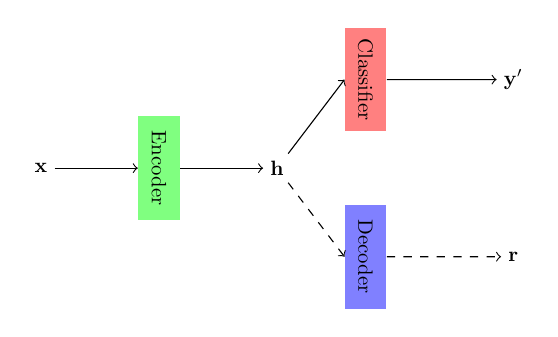
\begin{tikzpicture}[scale=0.75, every node/.style={scale=0.75}]
		\tikzstyle{block} = [rectangle,minimum width=5em,minimum height=2em]
		\node[rotate=270,block,fill=green!50]at (2,0.5)(encoder){Encoder};
		\node[](sentence)at (0,0.5){$\mathbf{x}$};
		\node[](p)at (8,2){$\mathbf{y}'$};
		\node[](r)at (8,-1){$\mathbf{r}$};
		\node[rotate=270,block,fill=red!50](classifier)at (5.5,2){Classifier};
		\node[rotate=270,block,fill=blue!50](decoder)at (5.5,-1){Decoder};
		\node[](c)at (4,0.5){$\mathbf{h}$};
		\path[->] (sentence) edge (encoder)
		(encoder)  edge (c)
		(c) edge (classifier.south)
		(classifier) edge (p);
		\path[->,dashed] (c) edge (decoder.south)
		(decoder) edge (r);
		\end{tikzpicture}
		\caption{Unsupervised pretaining by using autoencoder, the encoder is first pretrained as part of autoencoder (dashed line), and then tuned with a classifier (solid line).}
	\end{figure*}
	\section{Neural Language Models}
	\textbf{Neural language models} (\textbf{NLMs}) are members of neural networks for language modelling. 
	NLMs gained attentions after Bengio et al \cite{bengio2003neural} used a feedforward neural network to learn the representations for words in 2003. 
	However, until recently,  it was not possible to train an NLM efficiently on big amounts of data, because of hardware limitations, in Bengio et al\cite{bengio2003neural} also reported that they spend three weeks in training their model on forty CPUs for only five epochs. 
	With the recent advance in hardware development, researchers can train their neural network much more efficient on GPU.\\\\
	An NLM usually has following components in their model architecture\cite{collobert2008unified,collobert2011natural}
	\begin{enumerate}
		\item An embedding layer that allows NLM to perform index lookup and find corresponded feature vectors for the given input words. 
		The technique used to acquire feature vectors will be presented soon. 
		We will introduce how to create these indexes and embedding layer in our experiments later in section 4.1.2 and 4.1.3.
		\item An encoding neural network which takes the look-upped feature vectors as inputs and encodes them into intermediate hidden representations.
		Then the intermediate hidden representations are passed to an output classifier and perform a certain task.
	\end{enumerate}
		\begin{figure*}[h]
			\centering
			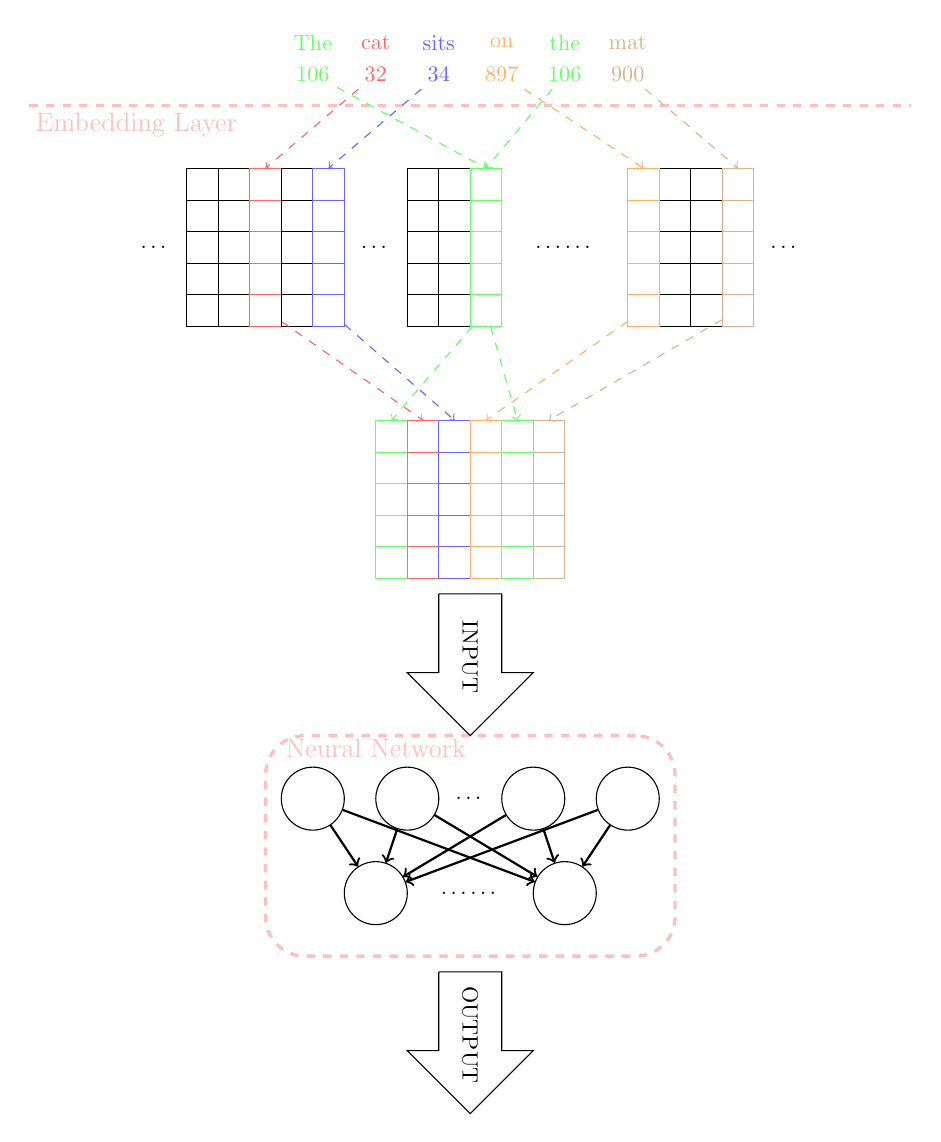
\begin{tikzpicture}[scale=0.8, every node/.style={scale=0.8}]
			\tikzstyle{ks} = [rectangle,minimum height=0.5cm,minimum width=0.5cm];
			\tikzstyle{neuron}=[circle,minimum size=1cm]
			\node[](w1)at(-2.5,7.5){\textcolor{green!60}{The}}; 
			\node[](w2)at(-1.5,7.5){\textcolor{red!60}{cat}};
			\node[](w3)at(-0.5,7.5){\textcolor{blue!60}{sits}};
			\node[](w4)at(0.5,7.5){\textcolor{orange!60}{on}};
			\node[](w5)at(1.5,7.5){\textcolor{green!60}{the}};
			\node[](w6)at(2.5,7.5){\textcolor{brown!60}{mat}};
			
			\node[](i1)at(-2.5,7){\textcolor{green!60}{106}}; 
			\node[](i2)at(-1.5,7){\textcolor{red!60}{32}};
			\node[](i3)at(-0.5,7){\textcolor{blue!60}{34}};
			\node[](i4)at(0.5,7){\textcolor{orange!60}{897}};
			\node[](i5)at(1.5,7){\textcolor{green!60}{106}};
			\node[](i6)at(2.5,7){\textcolor{brown!60}{900}};
			\draw[pink!,very thick, dashed]{
				(-7,6.5) -- (7,6.5)
			};
			\node[](title1)at(-5.3,6.2){\large\textcolor{pink}{Embedding Layer}};
			\foreach \j in {1,2}{
				\foreach \i in {1,...,5}{
					\node[draw,ks] at (\j*0.5-4.75,2.75+\i*0.5){};
					\node[draw,ks] at (\j*0.5+2.75,2.75+\i*0.5){};
					\node[draw,ks] at (\j*0.5-1.25,2.75+\i*0.5){};
				};	
			};
			
			\foreach \i in {1,...,5}{
				\node[draw=red!60,ks](r\i) at (-3.25,2.75+\i*0.5){};
				\node[draw,ks] at (-2.75,2.75+\i*0.5){};
				\node[draw=green!60,ks](g\i) at (0.25,2.75+\i*0.5){};
				\node[draw=blue!60,ks](b\i) at (-2.25,2.75+\i*0.5){};
				\node[draw=orange!60,ks](o\i) at (2.75,2.75+\i*0.5){};
				\node[draw=brown!60,ks](br\i) at (4.25,2.75+\i*0.5){};
			};	
			\node[]()at (-5,4.25){\dots};
			\node[]()at(-1.5,4.25){\dots};
			\node[]()at(1.5,4.25){\dots\dots};
			\node[]()at(5,4.25){\dots};
			\path[->,dashed,red!60] (i2) edge (r5.north);
			\path[->,dashed,blue!60] (i3) edge (b5.north);
			\path[->,dashed,green!60] (i1) edge (g5.north);
			\path[->,dashed,green!60] (i5) edge (g5.north);
			\path[->,dashed,orange!60] (i4) edge (o5.north);
			\path[->,dashed,brown!60] (i6) edge (br5.north);
			
			\foreach \i in {1,...,5}{
				\node[draw=green!60,ks](g\i\i) at (-1.25,-1.25+\i*0.5){};
				\node[draw=red!60,ks](r\i\i) at (-0.75,-1.25+\i*0.5){};
				\node[draw=blue!60,ks](b\i\i) at (-0.25,-1.25+\i*0.5){};
				\node[draw=orange!60,ks](o\i\i) at (0.25,-1.25+\i*0.5){};
				\node[draw=green!60,ks](g2\i\i) at (0.75,-1.25+\i*0.5){};
				\node[draw=brown!60,ks](br\i\i) at (1.25,-1.25+\i*0.5){};
			};
			
			\path[->,dashed,red!60] (r1) edge (r55.north);
			\path[->,dashed,blue!60] (b1) edge (b55.north);
			\path[->,dashed,green!60] (g1) edge (g55.north);
			\path[->,dashed,green!60] (g1) edge (g255.north);
			\path[->,dashed,orange!60] (o1) edge (o55.north);
			\path[->,dashed,brown!60] (br1) edge (br55.north);
			
			
			
			\node[draw,neuron](n1) at (-2.5,-4.5){};
			\node[draw,neuron](n2) at (-1,-4.5){};
			\node[draw,neuron](n3) at (1,-4.5){};
			\node[draw,neuron](n4) at (2.5,-4.5){};
			\node[draw,neuron](n5) at (-1.5,-6){};
			\node[draw,neuron](n6) at (1.5,-6){};
			\node[](title2)at(-1.5,-3.7){\large\textcolor{pink}{Neural Network}};
			\node [inner sep=0pt,minimum width=6.5cm,minimum height=3.5cm,outer sep=0pt,rounded corners=0.5cm,dashed,draw=pink,very thick] (pict) at (0,-5.25){};
			\path[->,thick] (n1) edge (n5)
			(n1) edge (n6)
			(n2) edge (n5)
			(n2) edge (n6)
			(n3) edge (n5)
			(n3) edge (n6)
			(n4) edge (n5)
			(n4) edge (n6);
			\node[]() at (0,-6){\dots\dots};
			\node[]() at (0,-4.5){\dots};
			\draw[]{
				(-0.5,-1.25) -- (0.5,-1.25) -- (0.5,-2.5) --(1,-2.5) -- (0,-3.5)
				--(-1,-2.5) --(-0.5,-2.5) --(-0.5,-1.25)
			};
			\draw[]{
				(-0.5,-7.25) -- (0.5,-7.25) -- (0.5,-8.5) --(1,-8.5) -- (0,-9.5)
				--(-1,-8.5) --(-0.5,-8.5) --(-0.5,-7.25)
			};
			\node[rotate=270]()at(0,-2.25){INPUT};
			\node[rotate=270]()at(0,-8.25){OUTPUT};
			\end{tikzpicture}
			\caption{Architecture of NLM's ,the word feature vectors are first retrieved from  embedding layer by index, then the feature vectors are fed into neural network to perform certain task.}
		\end{figure*}
		
	\subsection{Word Level Neural Language Model}
	Learning the vector representations for words from unlabelled data is one of the most successful applications of NLMs.
	There are some different word level NLMs have been proposed over the years\cite{mikolov2013distributed,pennington2014glove,morin2005hierarchical}. 
	Here we only briefly introduce \textbf{Continuous Bags of Words (CBOW)} proposed by Mikolov et al\cite{mikolov2013efficient}.\\\\
	The CBOW works as follow, given a small corpus `` There is a king lives in castle'',
	We first produce a central word and context pair $(\text{king},\{\text{ther is a lives in castle}\})$ and then give a one-hot vector to each word according to their orders in window
	\begin{align}
	\text{there} = \mathbf{v}_{1} = \begin{bmatrix}
	1\\0\\0\\0\\0\\0\\0\\
	\end{bmatrix} & &
	\text{is}= \mathbf{v}_{2} = \begin{bmatrix}
	0\\1\\0\\0\\0\\0\\0\\
	\end{bmatrix} & &
	\dots & &
	\text{castle} = \mathbf{v}_{7} = \begin{bmatrix}
	0\\0\\0\\0\\0\\0\\1
	\end{bmatrix}
	\end{align}
	We randomly initialise a matrix $\mathbf{W} \in \mathbb{R}^{7\times n}$ with in range $[-1,1]$, each word can obtain their corresponded word vector $\mathbf{w}_{i}$ by
	\begin{equation}
	\mathbf{w}_{i} = \mathbf{v}_{i}^{T}\mathbf{W}
	\end{equation} 
	Now we can set up a feedforward neural network takes $\mathbf{C} = \{\mathbf{w}_{1},\mathbf{w}_{2},\mathbf{w}_{3},\mathbf{w}_{5},\mathbf{w}_{6},\mathbf{w}_{7}\}$ as inputs, the first layer calculates the average $\mathbf{z}$ over $\mathbf{C}$
	\begin{equation}
		\mathbf{z} = \frac{1}{6}\sum_{w_{i}\in \mathbf{C}} \mathbf{w}_{i}
	\end{equation}
	The second layer of the neural network covert $\mathbf{z}$ into a seven dimensional vector $\mathbf{u}$
	\begin{equation}
		\mathbf{u} = \mathbf{z}^{T}\mathbf{U}
	\end{equation}
	The output layer is a softmax function computes the conditional probability 
	\begin{equation}
	p(\mathbf{w}_{i}|\mathbf{C}) = \frac{\exp(u_{i})}{\sum_{j=1}^{7}\exp(u_{j})}
	\end{equation}
	Where $\mathbf{w}_{i}\in\{\mathbf{w}_{1},\mathbf{w}_{2},\mathbf{w}_{3},\mathbf{w}_{4},\mathbf{w}_{5},\mathbf{w}_{6},\mathbf{w}_{7}\}$, $u_{i},u_{j}$ are elements of $\mathbf{u}$.
	Our target output is the central word ``king'', therefore the loss function is defined as
	\begin{equation}
	L = -\sum_{i=1}^{7}v_{4}^{i}p(\mathbf{w}_{i}|\mathbf{C})
	\end{equation}
	Where $v_{4}^{i}$ is $i$th element of $\mathbf{v}_{4}$.\\\\
	CBOW is incorporated with word2vec tool\footnote{https://code.google.com/archive/p/word2vec/}, which we will use to acquire word feature vectors for our experiments later.
	
	\subsection{Sentence Level Neural Language Model}
	Unlike word level NLMs, it is still not clear about which architectures or objectives can help us to learn the most useful sentences representations. 
	Nevertheless, there are still a few NLMs that can learn representations for sentences. For example
	\begin{itemize}
		\item \textbf{Recursive Autoencoder (RAE)}\cite{socher2011dynamic} is an autoencoder constructed based on the syntactic tree of a given input sentence. 
		Each node on the RAE encodes their children's output and provides the encoded vector to their parent's node. 
		We take the output of root node as the final representation of the sentence. 
		RAE can acquire more syntactical information about the sentence, as it is built from syntax tree. 
		But, to obtain high-quality syntax trees tremendous amount of pre-processing work is usually required.
		\item \textbf{Sequence to Sequence (seq2seq) Model}\cite{sutskever2014sequence,cho2014learning} consists of an encoding and a decoding RNN. The encoding RNN tries to encode intermediate representations from input data, while the decoding RNN produces sequences conditioned on the intermediate representations. Many applications of seq2seq model have observed that the learnt internal representations of seq2seq model can reflect some semantic meaning of input sentences.
		\item \textbf{Skip Through Vectors}\cite{kiros2015skip} can be consider as an extension of seq2seq model, given the consecutive sentences $S_{i-1}, S_{i}, S_{i+1}$, the Skip Through model encodes $S_{i}$ into an intermediate representation, and then predict $S_{i-1},S_{i+1}$ as outputs. 
		Training the Skip through vectors model must be able to access contextual information from consecutive sentences.
	\end{itemize}
	We can see that above models are developed based on different concepts. 
	A systematic comparison between these models has been made by Hill et al\cite{hill2016learning}. \\\\
	In this thesis, our primal interest is to study how different objectives can affect the sentence representations learnt by NLMs. 
	We do our experiments on seq2seq model mainly because of its ability to acquire representations for sentences without additional syntactic and contextual information. 
	In next chapter, We will discuss seq2seq model and how we set up this model to learn sentence representations in detail.
